\documentclass[10pt]{article}
\usepackage[margin=1in]{geometry}
\usepackage{booktabs}
\usepackage{amsmath}
\usepackage{amssymb}
\usepackage{multirow}
\usepackage{microtype}
\usepackage{tikz}
\usetikzlibrary{arrows.meta,positioning,fit,backgrounds}
\usepackage{subcaption}
\usepackage[hidelinks]{hyperref}

\title{\vspace{-2.5em}\textbf{Can Vision--Language--Action Models Forecast Bitcoin?\\
A Systematic Study of Target Normalization, Action-Head Architecture,\\ and Multi-Asset Design}}
\author{}
\date{}

\emergencystretch=1.5em
% --- float placement: let more floats share a page with text, avoid lone float pages ---
\setcounter{topnumber}{3}
\setcounter{bottomnumber}{2}
\setcounter{totalnumber}{5}
\renewcommand{\topfraction}{0.92}
\renewcommand{\bottomfraction}{0.85}
\renewcommand{\textfraction}{0.07}
\renewcommand{\floatpagefraction}{0.75}
\begin{document}
\maketitle
\vspace{-3.5em}

\begin{abstract}
\noindent
Vision--Language--Action (VLA) models excel at robot control, where a frozen vision--language
backbone conditions a diffusion action head. We ask whether this recipe transfers to a very
different domain: forecasting cryptocurrency prices. We adapt a GR00T/RLDX-style VLA
(Qwen3-VL backbone, flow-matching action head) to predict future Bitcoin (BTC) candles, and run
a \emph{controlled} four-axis ablation over (i)~target normalization, (ii)~action-head
architecture (single-stream cross-attention \emph{DiT} vs.\ multi-stream joint-attention
\emph{MSAT} from RLDX-1), (iii)~single- vs.\ multi-asset prediction, and (iv)~diffusion scope
(all-asset diffusion vs.\ BTC-only diffusion with read-off auxiliaries). Over a walk-forward
6-fold protocol (2020--2025) we find that (1)~\textbf{target normalization is the single most
important choice}: it cuts a regime-memorization index by ${\sim}3.7\times$ and reduces
price error (MAE) by 2--10$\times$, revealing that un-normalized models---including a previously
``best'' baseline---attain high directional accuracy only by memorizing each fold's trend;
(2)~\textbf{multi-asset context helps only under the joint-attention MSAT head}, and hurts under
DiT; and (3)~no from-scratch VLA beats buy-and-hold on average, while a \emph{pretrained}
time-series foundation model (Kronos) is the only model with positive returns on the clean
out-of-sample fold. Our study gives a systematic, honest map of what does and does not transfer,
and motivates pretraining and explicit uncertainty modeling for financial VLAs.
\end{abstract}

\vspace{-0.5em}
\section{Introduction}
VLA models unify perception, language, and action for robotics through a domain-agnostic recipe:
a frozen VLM produces latent tokens that condition a generative (diffusion / flow-matching)
action head. We test its transfer to \emph{financial time-series forecasting}---a domain with
weak signal, non-stationarity, and severe distribution shift.
\textbf{Contributions.} (1)~The first systematic application of a robot VLA architecture to
crypto forecasting. (2)~A confound-free \emph{four-axis} ablation isolating each design choice.
(3)~Quantification of a ``regime-memorization trap'': strong backtest metrics arising from trend
memorization rather than skill, exposed jointly by a long-ratio dispersion index and price MAE.
(4)~A head-to-head, contamination-controlled comparison against a pretrained foundation model
(Kronos).

\section{Related Work}
\textbf{Vision--Language--Action models} pair a (usually frozen) VLM with a generative action
head. Diffusion Policy~\cite{chi2023}, OpenVLA~\cite{openvla}, and GR00T/RLDX-1~\cite{rldx1}
establish the frozen-backbone $+$ diffusion-head recipe we adopt; flow matching~\cite{lipman2023}
is the generative objective, and RLDX-1~\cite{rldx1} contributes the multi-stream MSAT head we
compare against the single-stream DiT~\cite{peebles2023}.
\textbf{Time-series forecasting} has moved from specialized transformers (e.g.\
PatchTST~\cite{patchtst}) to \emph{pretrained} foundation models (Chronos~\cite{chronos}, and the
K-line model Kronos); our Kronos comparison directly probes this pretrained-vs.-from-scratch gap.
\textbf{Normalization against distribution shift} is standard in both fields: RevIN~\cite{revin}
reversibly normalizes time series, and robot action heads normalize actions by dataset
statistics---our per-asset target-std normalization is the crypto-delta analog, which we show is
decisive here.

\section{Method}
\textbf{Task.} Given the most recent 10 hourly candles, predict the next 12 candles as per-step
log-return deltas. The Qwen3-VL backbone is \emph{frozen}; only the action head trains
(Fig.~\ref{fig:arch}a).

\noindent\textbf{Flow-matching head.} The head learns a straight-line velocity field that
\emph{transports} Gaussian noise $\mathcal{N}(0,I)$ to the conditional distribution of future
price moves, i.e.\ diffusion-style generation. We compare two heads (Fig.~\ref{fig:arch}b):
\emph{DiT}~\cite{peebles2023}, a single-stream head that cross-attends to the VL tokens; and
\emph{MSAT}, the multi-stream head of RLDX-1~\cite{rldx1} (itself an action-modeling extension of
MM-DiT~\cite{esser2024}), which runs \emph{joint} self-attention over VL and action tokens so
that cross-asset structure can be modeled directly.

\noindent\textbf{Target normalization.} Flow-matching noise is unit-scale, but raw hourly deltas
are ${\sim}0.1\%$, so the signal is buried under the noise. We divide each asset's target delta
by its \emph{training-range} standard deviation (no look-ahead), matching the noise scale. This
is standard for robot action heads and for time-series models (e.g.\ RevIN); we treat it as an
ablation axis and un-normalize predictions at evaluation.

\noindent\textbf{Four design axes.} (i)~normalization on/off; (ii)~head DiT/MSAT; (iii)~assets
BTC vs.\ BTC+ETH+XRP; (iv)~diffusion scope: all assets diffused jointly (\emph{all-diff}) vs.\
BTC-only diffusion with ETH/XRP as auxiliary L1 ``read-off'' (RO) heads (unused at inference,
Fig.~\ref{fig:scope}).

\begin{figure}[t]
\centering
\begin{subcaptionblock}{0.53\textwidth}
\centering
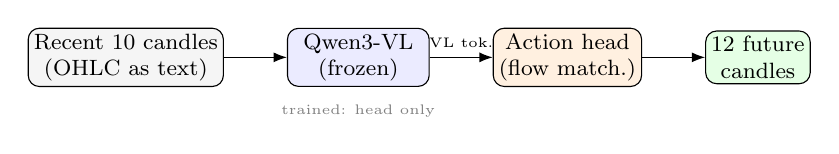
\begin{tikzpicture}[font=\footnotesize,node distance=4mm,
  box/.style={draw,rounded corners,minimum height=6.5mm,align=center,inner sep=2pt}]
\node[box,fill=gray!8] (txt) {Recent 10 candles\\(OHLC as text)};
\node[box,fill=blue!8,right=8mm of txt,minimum width=18mm] (vlm) {Qwen3-VL\\(frozen)};
\node[box,fill=orange!12,right=8mm of vlm,minimum width=18mm] (head) {Action head\\(flow match.)};
\node[box,fill=green!10,right=8mm of head] (out) {12 future\\candles};
\draw[-{Latex}] (txt) -- (vlm);
\draw[-{Latex}] (vlm) -- node[above,font=\tiny]{VL tok.} (head);
\draw[-{Latex}] (head) -- (out);
\node[below=1mm of vlm,font=\tiny,gray] {trained: head only};
\end{tikzpicture}
\caption{Pipeline}
\end{subcaptionblock}
\hfill
\begin{subcaptionblock}{0.44\textwidth}
\centering
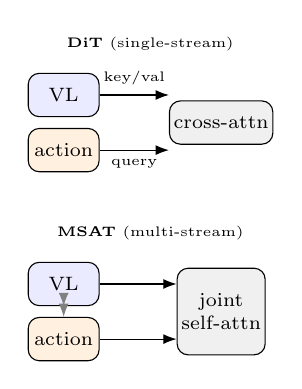
\begin{tikzpicture}[font=\scriptsize,
  b/.style={draw,rounded corners,minimum height=5.5mm,minimum width=9mm,align=center,inner sep=1.5pt}]
% ---- DiT (single-stream, cross-attention) ----
\node[font=\tiny] at (1.1,1.35) {\textbf{DiT} (single-stream)};
\node[b,fill=blue!8]   (vl1) at (0,0.7) {VL};
\node[b,fill=orange!12](a1)  at (0,0)   {action};
\node[b,fill=gray!12,minimum width=11mm] (dit) at (2.0,0.35) {cross-attn};
\draw[-{Latex}] (a1.east) -- node[below,font=\tiny]{query} (dit.west|-a1);
\draw[-{Latex}] (vl1.east) -- node[above,font=\tiny]{key/val} (dit.west|-vl1);
% ---- MSAT (multi-stream, joint self-attention) ----
\node[font=\tiny] at (1.1,-1.05) {\textbf{MSAT} (multi-stream)};
\node[b,fill=blue!8]   (vl2) at (0,-1.7) {VL};
\node[b,fill=orange!12](a2)  at (0,-2.4) {action};
\node[b,fill=gray!12,minimum width=11mm,minimum height=11mm] (msat) at (2.0,-2.05) {joint\\self-attn};
\draw[-{Latex}] (vl2.east) -- (msat.west|-vl2);
\draw[-{Latex}] (a2.east)  -- (msat.west|-a2);
\draw[{Latex}-{Latex},gray] (vl2.south) -- node[left,font=\tiny,xshift=-1pt]{} (a2.north);
\end{tikzpicture}
\caption{Action heads}
\end{subcaptionblock}
\caption{(a) A frozen VLM conditions a flow-matching action head that transports noise to future
price moves. (b) DiT cross-attends action tokens to VL tokens; MSAT jointly attends over both.}
\label{fig:arch}
\end{figure}

\begin{figure}[t]
\centering
\begin{subcaptionblock}{0.47\textwidth}
\centering
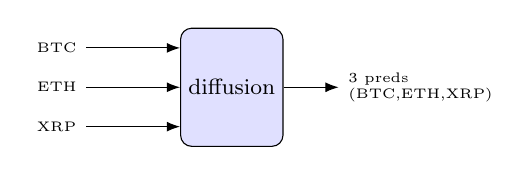
\begin{tikzpicture}[font=\footnotesize,
  b/.style={draw,rounded corners,minimum height=6mm,align=center,inner sep=2pt}]
\node[b,fill=blue!12,minimum width=13mm,minimum height=15mm] (d) at (2,0) {diffusion};
\foreach \y/\a in {0.5/BTC,0/ETH,-0.5/XRP}{%
  \draw[-{Latex}] (0.15,\y) node[left,font=\tiny]{\a} -- (d.west|-0,\y);}
\draw[-{Latex}] (d.east) -- ++(0.7,0) node[right,font=\tiny,align=left]{3 preds\\(BTC,ETH,XRP)};
\end{tikzpicture}
\caption{all-diff: all 3 assets jointly generated by diffusion.}
\end{subcaptionblock}
\hfill
\begin{subcaptionblock}{0.47\textwidth}
\centering
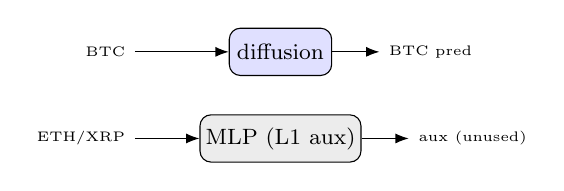
\begin{tikzpicture}[font=\footnotesize,
  b/.style={draw,rounded corners,minimum height=6mm,align=center,inner sep=2pt}]
\node[b,fill=blue!12,minimum width=13mm] (d) at (2,0.55) {diffusion};
\node[b,fill=gray!15,minimum width=13mm] (m) at (2,-0.55) {MLP (L1 aux)};
\draw[-{Latex}] (0.15,0.55) node[left,font=\tiny]{BTC} -- (d.west);
\draw[-{Latex}] (d.east) -- ++(0.6,0) node[right,font=\tiny]{BTC pred};
\draw[-{Latex}] (0.15,-0.55) node[left,font=\tiny]{ETH/XRP} -- (m.west);
\draw[-{Latex}] (m.east) -- ++(0.6,0) node[right,font=\tiny]{aux (unused)};
\end{tikzpicture}
\caption{read-off (RO): only BTC diffused; ETH/XRP as an L1 auxiliary, discarded at inference.}
\end{subcaptionblock}
\caption{\textbf{Axis (iv): diffusion scope.} Read-off treats ETH/XRP as a training-time
regularizer for BTC's representation rather than generating them. Under normalization, all-diff
wins (Table~\ref{tab:scope}).}
\label{fig:scope}
\end{figure}

\section{Experimental Setup}
Hourly OHLC for BTC/ETH/XRP, 2020--2025. \textbf{Walk-forward 6-fold}: each year, train Jan--Oct,
validate Nov, test Dec. All metrics are on BTC only.

\noindent\textbf{Metrics.} We report three metrics at a holding horizon of $k$ hours (a signal is
acted on and the position closed $k$ hours later); unless noted, all tables use $k{=}6$.
\emph{(1)~Directional accuracy} $\mathrm{DA}=\frac1N\sum_t\mathbf{1}[\hat r_{t,k}\,r_{t,k}>0]$,
the fraction of predictions whose sign matches the realized $k$-step return $r_{t,k}$
($\hat r_{t,k}$ is the prediction).
\emph{(2)~Return} (\textbf{ret}): we backtest a long-only rule---at each hour, if
$\hat r_{t,k}>\theta$ (a confidence gate), hold long for $k$ hours, else stay in cash. Because a
signal arrives every hour but each trade is held for $k$ hours, capital is split into $k$ slots
($1/k$ each) that trade at staggered offsets and compound independently; total exposure never
exceeds $100\%$ (no overlap leverage). We charge $0.1\%$ slippage per trade and report the
\emph{best} $\theta\!\in\!\{0.1,0.3,0.5,1.0\}\%$.
\emph{(3)~Abnormal excess return} (\textbf{AER})~$=\ \text{ret}-\text{ret}_{\text{B\&H}}$, where
$\text{ret}_{\text{B\&H}}$ is buy-and-hold (holding BTC over the test window); $\mathrm{AER}>0$
means the strategy beats passive holding.
As diagnostics we also report the regime index $\sigma$ (across-fold std of the long-ratio; low
is good) and close MAE (USD). We additionally evaluate a \emph{macro} variant (BTC + S\&P/
Treasuries, market-hours aligned) and \textbf{Kronos}, a pretrained K-line foundation model whose
June-2024 cutoff makes only the 2025 fold a clean out-of-sample (OOS) test.

\section{Results}
We present each axis as a controlled comparison---all other axes fixed---so effects are not
confounded (Tables~\ref{tab:head}--\ref{tab:norm}); all values are 6-fold averages at $k{=}6$.
Buy-and-hold over these folds returns ${+}7.1\%$, inflated by a single 2020 bull fold.

\begin{table}[htbp]
\centering
\begin{minipage}[t]{0.49\textwidth}
\centering\footnotesize
\caption{\textbf{Axes (i)+(ii): Assets $\times$ head} (norm on). Best head flips with asset
count; multi-asset only helps MSAT.}
\label{tab:head}
\begin{tabular}{llccc}
\toprule
Assets & Head & DA & ret & AER \\ \midrule
\multirow{2}{*}{single}
 & \textbf{DiT}  & 0.517 & \textbf{+0.040} & \textbf{$-$0.032} \\
 & MSAT          & 0.507 & +0.013 & $-$0.058 \\ \midrule
\multirow{2}{*}{multi}
 & DiT           & 0.512 & $-$0.013 & $-$0.085 \\
 & \textbf{MSAT} & 0.513 & \textbf{+0.027} & \textbf{$-$0.044} \\
\bottomrule
\end{tabular}\\[2pt]
{\footnotesize Single$\to$DiT, multi$\to$MSAT; ETH/XRP \emph{hurt} DiT, \emph{help} MSAT.}
\end{minipage}\hfill
\begin{minipage}[t]{0.49\textwidth}
\centering\footnotesize
\caption{\textbf{Axis (iii): Diffusion scope} (MSAT / 3-asset), for \emph{both} normalization
settings.}
\label{tab:scope}
\begin{tabular}{llccc}
\toprule
Norm & Scope & DA & ret & AER \\ \midrule
\multirow{2}{*}{on}
 & \textbf{all-diff} & 0.513 & \textbf{+0.027} & \textbf{$-$0.044} \\
 & read-off (RO)     & 0.504 & $-$0.003 & $-$0.074 \\ \midrule
\multirow{2}{*}{raw}
 & all-diff          & 0.523 & +0.016 & $-$0.055 \\
 & read-off (RO)$^\ast$ & 0.512 & +0.034 & $-$0.037 \\
\bottomrule
\end{tabular}\\[2pt]
{\footnotesize Under normalization, all-diff wins. $^\ast$RO's raw edge is regime
memorization ($\sigma{=}0.43$).}
\end{minipage}
\end{table}

\begin{table}[htbp]
\centering\small
\caption{\textbf{Axis (iv): Normalization} (MSAT / 3-asset / all-diff fixed). $\sigma$, MAE are
regime-trap diagnostics. Normalization cuts $\sigma$ $3.7\times$ and halves MAE at higher return.}
\label{tab:norm}
\begin{tabular}{lccccc}
\toprule
Norm & DA & ret & AER & $\sigma\!\downarrow$ & MAE$\downarrow$ \\ \midrule
\textbf{on}  & 0.513 & \textbf{+0.027} & \textbf{$-$0.044} & \textbf{0.111} & \textbf{580} \\
off (raw)    & 0.523 & +0.016 & $-$0.055 & 0.406 & 1096 \\
\bottomrule
\end{tabular}
\end{table}

\noindent\textbf{(i)~Assets and (ii)~head interact} (Table~\ref{tab:head}). The best head depends
on asset count (single$\to$DiT, multi$\to$MSAT), and adding ETH/XRP \emph{hurts} DiT
(ret $0.040\!\to\!-0.013$) but \emph{helps} MSAT ($0.013\!\to\!0.027$)---only MSAT's joint
attention exploits cross-asset structure. The best from-scratch setups are DiT-BTC and MSAT-Multi
(both normalized), yet both have AER${<}0$: on average \emph{nothing beats buy-and-hold}.

\noindent\textbf{(iii)~Diffusion scope} (Table~\ref{tab:scope}): how the auxiliary assets are
generated is secondary. Under normalization, jointly diffusing all assets beats the BTC-only
diffusion + ETH/XRP read-off auxiliary. Read-off appears stronger under raw targets, but only
because it inherits the same regime-memorization ($\sigma{=}0.43$) that inflates all un-normalized
models---not genuine skill.

\noindent\textbf{(iv)~Normalization is decisive} (Table~\ref{tab:norm}). Un-normalized heads
swing to the extremes---long-ratio ${\approx}1$ or ${\approx}0$ \emph{per fold}---memorizing that
fold's trend; their apparent edge is produced almost entirely by a single bull fold (2020), and
their price MAE degrades $2$--$10\times$ (up to 5497~USD for the previous baseline). \emph{High DA
or return without normalization is a mirage.} Table~\ref{tab:regime} makes the mechanism explicit:
the raw model's long-ratio collapses to ${\approx}1$ or ${\approx}0$ fold-by-fold (it simply
outputs each fold's dominant direction), whereas the normalized model stays moderate throughout.

\begin{table}[htbp]
\centering\small
\caption{\textbf{Regime-memorization trap}, per-fold long-ratio ($k{=}6$, MSAT / 3-asset). The raw
model bets ${\approx}100\%$ or ${\approx}0\%$ long \emph{per fold}, memorizing each fold's trend;
normalization keeps exposure moderate, so its edge generalizes rather than reflecting one bull fold.}
\label{tab:regime}
\begin{tabular}{lcccccc}
\toprule
Long-ratio by fold & 2020 & 2021 & 2022 & 2023 & 2024 & 2025 \\ \midrule
MSAT-Multi (norm) & 0.73 & 0.43 & 0.46 & 0.57 & 0.60 & 0.42 \\
MSAT-Multi (raw)  & 0.97 & \textbf{0.01} & \textbf{0.01} & 0.88 & 0.87 & 0.40 \\
\bottomrule
\end{tabular}
\end{table}

\noindent\textbf{Pretrained vs.\ from-scratch.} On the clean OOS fold (2025, a falling market),
\emph{no} from-scratch model earns positive returns (best DA ${\approx}0.51$), whereas pretrained
\textbf{Kronos} does (DA $0.534$; long-short returns up to $+5.9\%$ at $k{=}6$ and $+12.5\%$ at
$k{=}12$), despite never seeing 2025---while our models trained on 2025 Jan--Oct. A foundation
model generalizes where from-scratch VLA training does not (Table~\ref{tab:kronos}).

\begin{table}[htbp]
\centering\small
\caption{\textbf{Pretrained vs.\ from-scratch} on the clean OOS fold (2025, a falling market;
best-strategy return). Kronos never trained on 2025 yet is the \emph{only} profitable model, its
edge widening with horizon~$k$; our models trained \emph{on} 2025 Jan--Oct and still lose.}
\label{tab:kronos}
\begin{tabular}{lcccc}
\toprule
Model (fold 2025) & DA$_{k6}$ & ret$_{k6}$ & DA$_{k12}$ & ret$_{k12}$ \\ \midrule
DiT-BTC (from scratch)    & 0.489 & $-$0.014 & 0.495 & $+$0.003 \\
MSAT-Multi (from scratch) & 0.511 & $-$0.004 & 0.507 & $+$0.004 \\
\textbf{Kronos} (pretrained) & \textbf{0.534} & \textbf{$+$0.059} & \textbf{0.559} & \textbf{$+$0.125} \\ \midrule
Buy-and-hold              & --- & $-$0.053 & --- & $-$0.052 \\
\bottomrule
\end{tabular}
\end{table}

\noindent\textbf{Macro assets do not help} (Table~\ref{tab:macro}). On a separate market-hours-
aligned dataset, jointly predicting BTC with the S\&P~500 (SPY) and Treasuries of three maturities
(SHY~1--3\,yr, IEF~7--10\,yr, TLT~20\,yr$+$) never clearly beats the BTC-only baseline: DA is at or
below baseline for every macro variant, and the small differences are within noise (2 folds, 52
test samples). All AER${>}0$ only because this window is a down market ($\text{B\&H}{=}-6.2\%$).

\begin{table}[htbp]
\centering\small
\caption{\textbf{Macro variant} (DiT / all-diff / norm; 2-fold, market-hours aligned; $k{=}6$).
Adding S\&P/Treasuries does not improve BTC directional accuracy over the BTC-only baseline.}
\label{tab:macro}
\begin{tabular}{lccc}
\toprule
Co-predicted assets & DA & ret & AER \\ \midrule
baseline (BTC only)          & \textbf{0.465} & $-$0.031 & $+$0.032 \\
BTC + SPY + TLT (20\,yr$+$)  & 0.472 & $-$0.021 & \textbf{$+$0.042} \\
BTC + SPY + IEF (7--10\,yr)  & 0.363 & $-$0.036 & $+$0.026 \\
BTC + SPY + SHY (1--3\,yr)   & 0.419 & $-$0.028 & $+$0.034 \\
\bottomrule
\end{tabular}\\[2pt]
{\footnotesize Buy-and-hold over this window ${=}-6.2\%$; all ret${<}0$ (bearish 2024--25), so
positive AER reflects a falling benchmark, not skill.}
\end{table}

\section{Discussion}
Two metrics jointly diagnose the regime trap. The long-ratio dispersion $\sigma$ shows that a
model betting 100\% one way per fold cannot be deployed---its next-period direction is
unpredictable. Price MAE shows that such models are directionally ``lucky'' but numerically far
off. Normalization removes this pathology at no cost to genuine return. Across all axes, structural
choices \emph{among from-scratch models} only reallocate a weak signal---so the limiting factor is
not the VLA design but its lack of pretraining, exactly the advantage the pretrained baseline
enjoys. This points \emph{toward}, not away from, VLAs: the same architecture, given financial
pretraining and an explicit uncertainty head, is the natural way to convert that latent signal
into skill.

\section{Future Work and Conclusion}
\textbf{Action uncertainty via a learned confidence token.} Because the diffusion head is
stochastic, a natural extension is to let the model report \emph{how confident} it is. We will
grow the action sequence from 12 to 13 tokens, where the 13th token is trained as a \emph{learned
error/confidence head}: it predicts the model's own expected error (the residual between
predicted and realized moves), turning the network into its own uncertainty estimator. This
per-step confidence can then gate position sizing---trading only when calibrated confidence is
high---directly targeting risk-adjusted profitability. We further plan large-corpus pretraining
and reversible input normalization to counter distribution shift.

\noindent\textbf{Regime-aware modeling.} Our regime-memorization analysis exposes a deeper issue:
reporting or selecting a model \emph{per fold} amounts to cherry-picking, since each fold is
dominated by one market regime. Rather than fitting one model to a mixture of regimes (or picking
the fold that flatters it), a principled next step is a set of \emph{regime-specialized} policies
---bull, bear, and sideways (range-bound)---with an online regime classifier routing each period
to the matching expert. This directly attacks the pathology we quantify with $\sigma$: instead of
one model memorizing whichever regime a fold happens to be in, each expert learns behavior
appropriate to its regime, and routing (not memorization) supplies the directional prior.

\noindent\textbf{Limitations.} We fix the context length (10 text candles) and use a text-only
prompt (a chart-image input path exists but is disabled); a systematic ablation of context length
and of chart-image conditioning is left to future work, alongside longer test windows and
additional markets.

\noindent\textbf{Summary and ongoing work.} This study maps \emph{what transfers} when a robot VLA
is applied to financial forecasting. Three controlled findings---target normalization is decisive
(it dismantles a regime-memorization mirage), multi-asset context helps only under joint-attention
heads, and \emph{from-scratch training}---not the VLA architecture---is the limiting factor---show
where the remaining gains must come from. Far from abandoning VLAs, they chart how to \emph{advance}
one: my next steps are (i)~\emph{financial pretraining} of the VLA, mirroring the advantage the
pretrained baseline enjoys; (ii)~an explicit \emph{uncertainty head} (the 13th token) that lets the
model abstain when it cannot predict; and (iii)~\emph{regime-specialized} experts with online
routing. I treat this controlled, honestly-negative result not as an endpoint but as the groundwork
that makes a stronger financial VLA concrete and testable.

\begin{thebibliography}{9}
\small
\bibitem{rldx1} D.~Kim, H.~Jang, M.~Koo, et al. (RLWRLD). RLDX-1 Technical Report.
\emph{arXiv:2605.03269}, 2026.
\bibitem{peebles2023} W.~Peebles and S.~Xie. Scalable Diffusion Models with Transformers (DiT).
\emph{ICCV}, 2023.
\bibitem{esser2024} P.~Esser et al. Scaling Rectified Flow Transformers for High-Resolution Image
Synthesis (MM-DiT). \emph{ICML}, 2024.
\bibitem{chi2023} C.~Chi et al. Diffusion Policy: Visuomotor Policy Learning via Action Diffusion.
\emph{RSS}, 2023.
\bibitem{openvla} M.~J.~Kim et al. OpenVLA: An Open-Source Vision-Language-Action Model.
\emph{CoRL}, 2024.
\bibitem{lipman2023} Y.~Lipman et al. Flow Matching for Generative Modeling. \emph{ICLR}, 2023.
\bibitem{patchtst} Y.~Nie et al. A Time Series is Worth 64 Words: Long-Term Forecasting with
Transformers. \emph{ICLR}, 2023.
\bibitem{chronos} A.~F.~Ansari et al. Chronos: Learning the Language of Time Series.
\emph{TMLR}, 2024.
\bibitem{revin} T.~Kim et al. Reversible Instance Normalization for Accurate Time-Series
Forecasting against Distribution Shift. \emph{ICLR}, 2022.
\end{thebibliography}

\end{document}
